\section{Introducción}\label{intro}
\subsection{¿Qué es Moogle?}
\begin{frame}
    \centering
    {\large ¿Qué es Moogle?\par}
    \vspace{.5cm}

    \pause
    \begin{figure}
    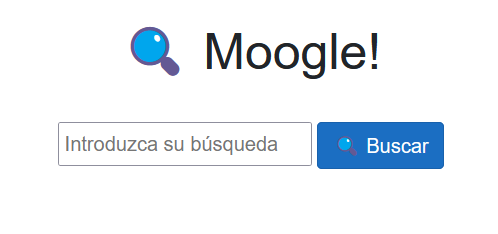
\includegraphics[width=5cm]{sections/moog.png}
    \end{figure}
    {\large Moogle es una interfaz web creada con el fin de buscar
    un texto en un grupo de archivos. Para su funcionamiento
    utiliza un Sistema de Recuperación de Información
    desarrollado en lenguaje $C\#$}   


\end{frame}